% Change to 'masters' to produces the masters thesis preliminary pages
\documentclass[oneside,honors,etd]{WSUclass}

\usepackage{import}

% preamble contains title page, signature page, acknowledgment and abstract texts
\usepackage{preamble}

% Packages used
\usepackage[utf8]{inputenc} % Remove warning on ascii conversion
\usepackage[T1]{fontenc} % Remove warning on ascii conversion
\usepackage[refsection=part,citestyle=apa,style=authoryear,natbib=true,backend=biber]{biblatex}
\usepackage{hyperref}

% Make chapter numbers into string words 1 -> ONE
\usepackage{fmtcount}
\makeatletter
\renewcommand{\@makechapterhead}[1]{\vspace *{40\p@ }{\parindent \z@ 
\raggedright \normalfont \ifnum \c@secnumdepth >\m@ne \Huge \bfseries 
\@chapapp \space \Numberstring{chapter} \vskip 10\p@ \fi #1\par \nobreak \vskip 30\p@ }}
\makeatother

\addbibresource{bib.bib}

\begin{document}

\hypersetup{breaklinks=true}

 % Start page counting in roman numerals
 \frontmatter

 % This command makes the formal preliminary pages.
 % You can comment it out during the drafting process if you want to save paper.
 \makepreliminarypages

 \doublespace
 % Make the table of contents.
 \tableofcontents
 \thispagestyle{plain}

 % Make the list of tables
 \mylistoftables
 \thispagestyle{plain}
 
 % Make the list of figures
 \mylistoffigures
 \thispagestyle{plain}

  % This page is OPTIONAL. To remove, comment out and \dedicationpage in diss.tex
 \dedicationpage
 \clearemptydoublepage

 % Start regular page counting at page 1
 \mainmatter

% OK. Everything is set up. Type your thesis here.
\addchapheadtotoc
\chapter{INTRODUCTION}

\section{Why digital marketplaces are important}
Digital marketplaces shape our modern economy and the way people connect for goods and services. They exist in great variety and prevalence in day-to-day life. Many consumers interact with these marketplaces unknowingly, as the good or service is, deliberately, branded and commodified. Despite their outward simplicity, digital marketplaces like Uber and Instacart contain an enormous amount of complexity managing suppliers and organizing the provision of their respective services. The decisions that digital marketplaces make carry real weight and affect lives at an unprecedented scale.

\section{Economic value and impact created in digital marketplaces}
Marketplaces have been heralded as the "Fourth Wave" of Ecommerce, and are projected to grow by trillions of dollars in the years to come \citep{marketplaceBoom}. Marketplace businesses create enormous value by connecting people for value exchange and lowering the costs associated with transacting. By aggregating suppliers and buyers, marketplaces can regulate quality and commodify services, providing more value to each side of the market while netting large profits. Furthermore, these digital marketplaces are hugely defensible as they benefit from a network effect, making the platforms increasingly difficult to disrupt as they grows in each market.

\section{Types of digital marketplaces}

There is an evolving vernacular around marketplaces. The field is broad and covers a number of different types of businesses. In this paper, I will reduce digital marketplaces into two categories: Diversified Marketplaces and Commodified Marketplaces. 

\subsection{Diversified Marketplaces}
Diversified Marketplaces sell many goods to their users. Amazon, Alibaba, and eBay are examples of diversified marketplaces. These marketplaces offer variety, trust, and convenience to consumers.

\subsection{Commodified Marketplaces}
Commodified Marketplaces, the focus of this paper, sell a specific service (or set of services) to consumers. Each service is commodified and priced independent of which supplier ultimately provides the service. For example, Uber gives you a price estimate based on the ride (the service) not the driver (the supplier). Commodified marketplaces like Uber and Instacart offer services to consumers without the complication of who or how. These marketplaces are opaque by design, streamlining the provision of the service and shielding consumers from the details. They also tend to focus on niche services in order to polish the user experience. For example, Wag commodified dog walks.

\begin{table}
  \begin{center}
  \begin{tabular}{|l|p{4cm}|c|c|}
  \hline
  {\sc Name}  &  {\sc Description} & {\sc Classification} & {\sc URL} \\
  \hline
  Amazon          & Online seller of almost anything & Diversified & \url{https://amazon.com} \\
  \hline
  Uber      & On-demand rides & Commodified & \url{https://uber.com} \\
  \hline
  Instacart    & Grocery delivery & Commodified & \url{https://instacart.com} \\
  \hline
  Wag!  & Pet services & Commodified & \url{https://wagwalking.com} \\
  \hline
  DoorDash  & Food delivery & Commodified & \url{https://doordash.com} \\
  \hline
  lugg  & Move anything with the tap of a button & Commodified & \url{https://lugg.com} \\
  \hline
  Thumbtack  & Find a local pro for pretty much anything & Diversified & \url{https://thumbtack.com} \\
  \hline
  \end{tabular}
  \end{center}
  \caption{Examples of Digital Marketplaces}
  \label{digital_marketplaces}
  \end{table}

\section{Changing definition of work and the gig economy}
Work is changing as our economy evolves. More and more people are employed in the gig economy, working flexible hours under the umbrella of some digital marketplace. Instead of working for a taxi company, drivers are providing rides through Uber. With this transition, service providers are reorganizing and the incentive structures must be re-evaluated. As a result of this reorganization, many workers are losing protections that were once considered essential, such as healthcare and severance.

\section{Power of a platform to organize economic activity}
The macroeconomic shift to the gig economy and the enormous value creation and provision from digital markeplaces highlight the power that these platforms have to organize economic activity and the wellbeing of millions (maybe billions) of people. These platforms are immensely powerful – they shape the very fabric of our economy. This is especially true in The United States, where in 2017 Services made up over 77\% of the economy \citep{economyDistribution}.

\section{Research landscape}
Despite their significance and relevance, digital marketplaces are still a relatively new phenomenon, and much research remains underdeveloped. Successful digital marketplaces like Uber have created large teams of economists in an attempt to optimize their operations, but their inquiry is specific to their individual challenges. This paper is intended to provide a reductionist theory and some practical considerations that can be broadly applied to commodified digital marketplaces.
\chapter{COMMODIFIED DIGITAL MARKETPLACE THEORY}
\section{Precursor}
Example of hyperlink \url{http://www.wikibooks.org}. Fusce ultricies pulvinar diam sed ultrices. Sed orci justo, rutrum in dolor a, consequat dictum mi. Sed luctus congue ex nec dignissim. Phasellus volutpat urna vestibulum ipsum vestibulum, quis venenatis justo consectetur. Nullam hendrerit nisl in rutrum convallis. Sed sit amet malesuada nisi. Phasellus dolor neque, vehicula vestibulum semper at, facilisis eget libero. Mauris interdum magna molestie, auctor felis a, condimentum odio. Pellentesque habitant morbi tristique senectus et netus et malesuada fames ac turpis egestas. Suspendisse maximus lacinia dignissim. Maecenas pharetra accumsan metus, sagittis dictum purus sollicitudin eget. Curabitur ut porttitor arcu, ut porttitor ipsum. Vestibulum porttitor finibus sapien, ac pharetra odio bibendum nec. Nullam tincidunt dignissim risus imperdiet dictum.

Pellentesque habitant morbi tristique senectus et netus et malesuada fames ac turpis egestas. Suspendisse maximus lacinia dignissim. Maecenas pharetra accumsan metus, sagittis dictum purus sollicitudin eget. Curabitur ut porttitor arcu, ut porttitor ipsum. Vestibulum porttitor finibus sapien, ac pharetra odio bibendum nec. Nullam tincidunt dignissim risus imperdiet dictum.

\subsection{Background}
Another example of hyperlink \href{http://www.wikibooks.org}{Wikibooks home}. Nullam mollis et leo at pharetra. Nulla efficitur molestie euismod. Sed dapibus metus sed tempus varius. Aenean finibus eros ut urna luctus feugiat. Duis turpis risus, viverra vitae porta et, ullamcorper ac est. Proin in eros nec ipsum interdum tempus. Nam fringilla lectus velit, non posuere ex vehicula ut. Mauris tincidunt, dolor sit amet commodo tempor, erat mi egestas dui, at elementum tellus est rhoncus libero. Ut et rutrum lectus, id viverra tortor. Vivamus nec lacus eros. Donec dictum porta nisi et vestibulum. Mauris luctus ligula ut libero aliquet luctus. Quisque malesuada egestas finibus.

\subsection{Proposed definition}
Another example of hyperlink \href{http://www.wikibooks.org}{Wikibooks home}. Nullam mollis et leo at pharetra. Nulla efficitur molestie euismod. Sed dapibus metus sed tempus varius. Aenean finibus eros ut urna luctus feugiat. Duis turpis risus, viverra vitae porta et, ullamcorper ac est. Proin in eros nec ipsum interdum tempus. Nam fringilla lectus velit, non posuere ex vehicula ut. Mauris tincidunt, dolor sit amet commodo tempor, erat mi egestas dui, at elementum tellus est rhoncus libero. Ut et rutrum lectus, id viverra tortor. Vivamus nec lacus eros. Donec dictum porta nisi et vestibulum. Mauris luctus ligula ut libero aliquet luctus. Quisque malesuada egestas finibus.

\section{Model}

\subsection{Setup and Assumptions}
Pellentesque habitant morbi tristique senectus et netus et malesuada fames ac turpis egestas. Suspendisse maximus lacinia dignissim. Maecenas pharetra accumsan metus, sagittis dictum purus sollicitudin eget. Curabitur ut porttitor arcu, ut porttitor ipsum. Vestibulum porttitor finibus sapien, ac pharetra odio bibendum nec. Nullam tincidunt dignissim risus imperdiet dictum.

\subsection{Definitions}
Pellentesque habitant morbi tristique senectus et netus et malesuada fames ac turpis egestas. Suspendisse maximus lacinia dignissim. Maecenas pharetra accumsan metus, sagittis dictum purus sollicitudin eget. Curabitur ut porttitor arcu, ut porttitor ipsum. Vestibulum porttitor finibus sapien, ac pharetra odio bibendum nec. Nullam tincidunt dignissim risus imperdiet dictum.

\subsubsection{Good/Service}
Pellentesque habitant morbi tristique senectus et netus et malesuada fames ac turpis egestas. Suspendisse maximus lacinia dignissim. Maecenas pharetra accumsan metus, sagittis dictum purus sollicitudin eget. Curabitur ut porttitor arcu, ut porttitor ipsum. Vestibulum porttitor finibus sapien, ac pharetra odio bibendum nec. Nullam tincidunt dignissim risus imperdiet dictum.

\subsubsection{Suppliers}
Pellentesque habitant morbi tristique senectus et netus et malesuada fames ac turpis egestas. Suspendisse maximus lacinia dignissim. Maecenas pharetra accumsan metus, sagittis dictum purus sollicitudin eget. Curabitur ut porttitor arcu, ut porttitor ipsum. Vestibulum porttitor finibus sapien, ac pharetra odio bibendum nec. Nullam tincidunt dignissim risus imperdiet dictum.

\subsubsection{Quality}
Pellentesque habitant morbi tristique senectus et netus et malesuada fames ac turpis egestas. Suspendisse maximus lacinia dignissim. Maecenas pharetra accumsan metus, sagittis dictum purus sollicitudin eget. Curabitur ut porttitor arcu, ut porttitor ipsum. Vestibulum porttitor finibus sapien, ac pharetra odio bibendum nec. Nullam tincidunt dignissim risus imperdiet dictum.

\subsubsection{Price}
Pellentesque habitant morbi tristique senectus et netus et malesuada fames ac turpis egestas. Suspendisse maximus lacinia dignissim. Maecenas pharetra accumsan metus, sagittis dictum purus sollicitudin eget. Curabitur ut porttitor arcu, ut porttitor ipsum. Vestibulum porttitor finibus sapien, ac pharetra odio bibendum nec. Nullam tincidunt dignissim risus imperdiet dictum.

\subsubsection{Demand}
Pellentesque habitant morbi tristique senectus et netus et malesuada fames ac turpis egestas. Suspendisse maximus lacinia dignissim. Maecenas pharetra accumsan metus, sagittis dictum purus sollicitudin eget. Curabitur ut porttitor arcu, ut porttitor ipsum. Vestibulum porttitor finibus sapien, ac pharetra odio bibendum nec. Nullam tincidunt dignissim risus imperdiet dictum.

\subsubsection{Marketplace}
Pellentesque habitant morbi tristique senectus et netus et malesuada fames ac turpis egestas. Suspendisse maximus lacinia dignissim. Maecenas pharetra accumsan metus, sagittis dictum purus sollicitudin eget. Curabitur ut porttitor arcu, ut porttitor ipsum. Vestibulum porttitor finibus sapien, ac pharetra odio bibendum nec. Nullam tincidunt dignissim risus imperdiet dictum.

\subsection{Solving the model}
Pellentesque habitant morbi tristique senectus et netus et malesuada fames ac turpis egestas. Suspendisse maximus lacinia dignissim. Maecenas pharetra accumsan metus, sagittis dictum purus sollicitudin eget. Curabitur ut porttitor arcu, ut porttitor ipsum. Vestibulum porttitor finibus sapien, ac pharetra odio bibendum nec. Nullam tincidunt dignissim risus imperdiet dictum.

\subsection{Trade-offs}
Pellentesque habitant morbi tristique senectus et netus et malesuada fames ac turpis egestas. Suspendisse maximus lacinia dignissim. Maecenas pharetra accumsan metus, sagittis dictum purus sollicitudin eget. Curabitur ut porttitor arcu, ut porttitor ipsum. Vestibulum porttitor finibus sapien, ac pharetra odio bibendum nec. Nullam tincidunt dignissim risus imperdiet dictum.

\section{Conclusions}

\subsection{Borrowing Constraint}
Pellentesque habitant morbi tristique senectus et netus et malesuada fames ac turpis egestas. Suspendisse maximus lacinia dignissim. Maecenas pharetra accumsan metus, sagittis dictum purus sollicitudin eget. Curabitur ut porttitor arcu, ut porttitor ipsum. Vestibulum porttitor finibus sapien, ac pharetra odio bibendum nec. Nullam tincidunt dignissim risus imperdiet dictum.

\subsection{Runaway Markets}
Pellentesque habitant morbi tristique senectus et netus et malesuada fames ac turpis egestas. Suspendisse maximus lacinia dignissim. Maecenas pharetra accumsan metus, sagittis dictum purus sollicitudin eget. Curabitur ut porttitor arcu, ut porttitor ipsum. Vestibulum porttitor finibus sapien, ac pharetra odio bibendum nec. Nullam tincidunt dignissim risus imperdiet dictum.

\subsection{Gamblers' Markets}
Pellentesque habitant morbi tristique senectus et netus et malesuada fames ac turpis egestas. Suspendisse maximus lacinia dignissim. Maecenas pharetra accumsan metus, sagittis dictum purus sollicitudin eget. Curabitur ut porttitor arcu, ut porttitor ipsum. Vestibulum porttitor finibus sapien, ac pharetra odio bibendum nec. Nullam tincidunt dignissim risus imperdiet dictum.

\subsubsection{Under Monopoly}
Pellentesque habitant morbi tristique senectus et netus et malesuada fames ac turpis egestas. Suspendisse maximus lacinia dignissim. Maecenas pharetra accumsan metus, sagittis dictum purus sollicitudin eget. Curabitur ut porttitor arcu, ut porttitor ipsum. Vestibulum porttitor finibus sapien, ac pharetra odio bibendum nec. Nullam tincidunt dignissim risus imperdiet dictum.

\subsubsection{Under Competition}
Pellentesque habitant morbi tristique senectus et netus et malesuada fames ac turpis egestas. Suspendisse maximus lacinia dignissim. Maecenas pharetra accumsan metus, sagittis dictum purus sollicitudin eget. Curabitur ut porttitor arcu, ut porttitor ipsum. Vestibulum porttitor finibus sapien, ac pharetra odio bibendum nec. Nullam tincidunt dignissim risus imperdiet dictum.

\subsection{Marketplace Stages}

\subsubsection{Setup}
Pellentesque habitant morbi tristique senectus et netus et malesuada fames ac turpis egestas. Suspendisse maximus lacinia dignissim. Maecenas pharetra accumsan metus, sagittis dictum purus sollicitudin eget. Curabitur ut porttitor arcu, ut porttitor ipsum. Vestibulum porttitor finibus sapien, ac pharetra odio bibendum nec. Nullam tincidunt dignissim risus imperdiet dictum.

\subsubsection{Early Stage}
Pellentesque habitant morbi tristique senectus et netus et malesuada fames ac turpis egestas. Suspendisse maximus lacinia dignissim. Maecenas pharetra accumsan metus, sagittis dictum purus sollicitudin eget. Curabitur ut porttitor arcu, ut porttitor ipsum. Vestibulum porttitor finibus sapien, ac pharetra odio bibendum nec. Nullam tincidunt dignissim risus imperdiet dictum

\subsubsection{Medium Stage}
Pellentesque habitant morbi tristique senectus et netus et malesuada fames ac turpis egestas. Suspendisse maximus lacinia dignissim. Maecenas pharetra accumsan metus, sagittis dictum purus sollicitudin eget. Curabitur ut porttitor arcu, ut porttitor ipsum. Vestibulum porttitor finibus sapien, ac pharetra odio bibendum nec. Nullam tincidunt dignissim risus imperdiet dictum

\subsubsection{Mature Stage}
Pellentesque habitant morbi tristique senectus et netus et malesuada fames ac turpis egestas. Suspendisse maximus lacinia dignissim. Maecenas pharetra accumsan metus, sagittis dictum purus sollicitudin eget. Curabitur ut porttitor arcu, ut porttitor ipsum. Vestibulum porttitor finibus sapien, ac pharetra odio bibendum nec. Nullam tincidunt dignissim risus imperdiet dictum

\section{Applications of Commodified Digital Marketplace Theory}

\subsection{Setup}
Pellentesque habitant morbi tristique senectus et netus et malesuada fames ac turpis egestas. Suspendisse maximus lacinia dignissim. Maecenas pharetra accumsan metus, sagittis dictum purus sollicitudin eget. Curabitur ut porttitor arcu, ut porttitor ipsum. Vestibulum porttitor finibus sapien, ac pharetra odio bibendum nec. Nullam tincidunt dignissim risus imperdiet dictum.

\subsection{Uber}
Pellentesque habitant morbi tristique senectus et netus et malesuada fames ac turpis egestas. Suspendisse maximus lacinia dignissim. Maecenas pharetra accumsan metus, sagittis dictum purus sollicitudin eget. Curabitur ut porttitor arcu, ut porttitor ipsum. Vestibulum porttitor finibus sapien, ac pharetra odio bibendum nec. Nullam tincidunt dignissim risus imperdiet dictum


\section{Model Extensions}

\subsection{Non-linear supplier acquisition cost}
Pellentesque habitant morbi tristique senectus et netus et malesuada fames ac turpis egestas. Suspendisse maximus lacinia dignissim. Maecenas pharetra accumsan metus, sagittis dictum purus sollicitudin eget. Curabitur ut porttitor arcu, ut porttitor ipsum. Vestibulum porttitor finibus sapien, ac pharetra odio bibendum nec. Nullam tincidunt dignissim risus imperdiet dictum.

\subsection{Variable quality}
Pellentesque habitant morbi tristique senectus et netus et malesuada fames ac turpis egestas. Suspendisse maximus lacinia dignissim. Maecenas pharetra accumsan metus, sagittis dictum purus sollicitudin eget. Curabitur ut porttitor arcu, ut porttitor ipsum. Vestibulum porttitor finibus sapien, ac pharetra odio bibendum nec. Nullam tincidunt dignissim risus imperdiet dictum.

\subsection{Goods versus services}
Pellentesque habitant morbi tristique senectus et netus et malesuada fames ac turpis egestas. Suspendisse maximus lacinia dignissim. Maecenas pharetra accumsan metus, sagittis dictum purus sollicitudin eget. Curabitur ut porttitor arcu, ut porttitor ipsum. Vestibulum porttitor finibus sapien, ac pharetra odio bibendum nec. Nullam tincidunt dignissim risus imperdiet dictum.

\subsection{How do you actually acquire new supply or demand}
Pellentesque habitant morbi tristique senectus et netus et malesuada fames ac turpis egestas. Suspendisse maximus lacinia dignissim. Maecenas pharetra accumsan metus, sagittis dictum purus sollicitudin eget. Curabitur ut porttitor arcu, ut porttitor ipsum. Vestibulum porttitor finibus sapien, ac pharetra odio bibendum nec. Nullam tincidunt dignissim risus imperdiet dictum.

\subsection{Marketplace chooses price}

\subsubsection{Demand as a function of price}
Pellentesque habitant morbi tristique senectus et netus et malesuada fames ac turpis egestas. Suspendisse maximus lacinia dignissim. Maecenas pharetra accumsan metus, sagittis dictum purus sollicitudin eget. Curabitur ut porttitor arcu, ut porttitor ipsum. Vestibulum porttitor finibus sapien, ac pharetra odio bibendum nec. Nullam tincidunt dignissim risus imperdiet dictum.


\subsubsection{Supply as a function of price}
Pellentesque habitant morbi tristique senectus et netus et malesuada fames ac turpis egestas. Suspendisse maximus lacinia dignissim. Maecenas pharetra accumsan metus, sagittis dictum purus sollicitudin eget. Curabitur ut porttitor arcu, ut porttitor ipsum. Vestibulum porttitor finibus sapien, ac pharetra odio bibendum nec. Nullam tincidunt dignissim risus imperdiet dictum.

\chapter{DIGITAL MARKETPLACES IN PRACTICE}
\section{Introduction}

In practice, digital marketplace are always unique and have their own product insights that make them successful. This theoretical model is not a prescription for digital marketplaces but rather a framework with which to think about the incentives at play in commodified digital marketplaces. To augment the CDM framework, this paper also explores the practical side of launching and growing digital marketplaces based on my personal research and experience.

\subsection{How the theory fails}.

This theory fails in more ways than one, but here are a few notable departures from practice.

\subsubsection{Market for the service may not exist}

The model assumes that a market for the service already exists, but in practice determining whether the market exists for a service is a large part of reaching product-market fit and cannot be assumed.

\subsubsection{There may not be sufficient supply in the market}

Even if there is a market for a given service, and you could commodify it using technology, there may not be sufficient supply in the market to create a successful commodified digital marketplace. If you wanted to build an on-demand service for disinfecting spaces, there may be sufficient demand and technology, but there may not be enough individuals or companies that want to engage in that service.

\subsection{Real-world challenges of a digital marketplace}

Departing from the CDM model entirely, there are a number of well-documented challenges that digital marketplaces face that are worth noting.

\section{Chicken and the Egg Problem}

Probably the most profound challenge is the chicken and the egg problem. Digital marketplaces are difficult to start because they require two different audiences to be orchestrated together. You need suppliers to attract buyers and buyers to attrack suppliers, but which comes first? Based on research into this topic, here are the top few strategies \citep{whatsNext}.

\subsection{Standalone Mode}

Standalone mode is when the product stands on its own without the marketplace. The product is usually made for one side of the market first, then after attracting users it opens up the marketplace. Users come to the product initially for the standalone mode, and their activity is used to launch a liquid marketplace. An example of this is LinkedIn (a marketplace between workers and companies) starting as a place for people to put their online CV and build their professional network. Similarly, Hire a Student lets students create their work profiles and showcase their work capacity, adding value to students in a market before there are hirers. Another example is OpenTable, which starts off selling reservation software to restaurants in a given market, then opens up the marketplace to diners when the market has sufficient restaurant density.

\subsection{Offering to fill empty seats for suppliers}

Another strategy to solve the chicken and egg problem is to build the market with existing, excess supply. This way, the supply is relatively easy to collect with the promise of incremental revenue.

\subsection{Buyers are sellers}

Another notable way to solve the chicken and egg problem is to make a digital marketplace where buyers are sellers. This way, the marketplace can focus on one target audience and build both sides of the market. This strategy makes it easier to match demand to supply and achieve market liquidity early. An example of this type of digital marketplace is OfferUp \url{https://offerup.com}. 

\section{Hacking Growth}

Another crucial element of any digital marketplace is how they hack growth. A clever growth hack can dramatically lower the cost to acquire new users and kickstart market liquidity.

\subsection{Referral}

One strategy is referral, whereby users are incentivized to refer other users. When I first launched Hire a Student, I created an advocacy program where students earned commission on other student signups. In the first week of launch, I was able to signup several hundred students (nearly 1/3 students at the school) using the referral program.
Over the past few years I have refined the referral program to be a consistent driver of user growth.

\begin{figure}[ht!]
\begin{center}
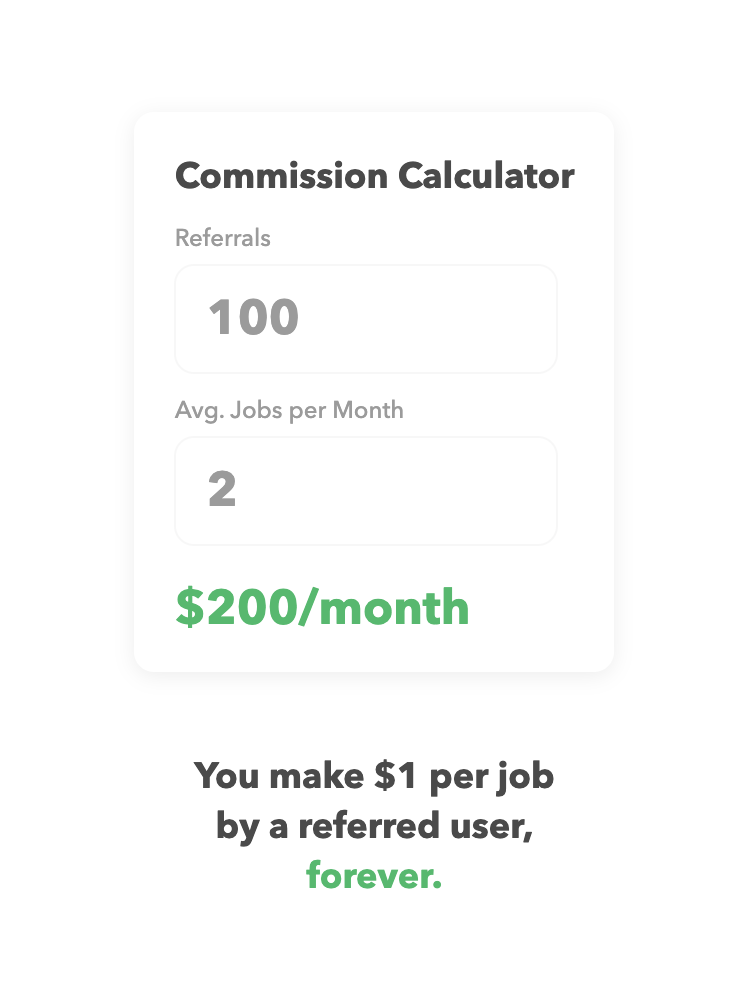
\includegraphics[scale=0.5]{figures/referral.png}
\end{center}
\caption[Example Referral Mechanism]{Hire a Student incentivizes users to refer others}
\label{referral}
\end{figure}

\subsection{Social}

Another strategy is to make the product social, creating no-cost incentives for users to share the app with their friends. Snackpass (\url{https://snackpass.co}), a Yale startup that lets users order food ahead and share rewards with friends, uses sharing rewards with friends as a viral social hook to attract and retain users.

\subsection{Network graphing}

Finally, there are a number of existing networks onto which new digital marketplaces can graph. For example, when launching Hire a Student, I found several local Facebook groups where community members exchanged recommendations for household services. Posting and commenting in these Facebook groups proved one of the highest impact channels.



% Bibliography
\begingroup
    \setlength\bibitemsep{10pt}
    \linespread{1}\selectfont
    \printbibliography[title=REFERENCES]
\endgroup
\addcontentsline{toc}{part}{REFERENCES}

% Appendices
\appendix

%%%%%%%%%% DON'T DELETE THIS, REVERTS NUMBERING BACK %%%%%%%%%%%%%
\makeatletter
\renewcommand{\@makechapterhead}[1]{\vspace *{-10\p@ }{\parindent \z@ 
\raggedright \normalfont \ifnum \c@secnumdepth >\m@ne \Huge \bfseries 
\@chapapp \space \thechapter \vskip 10\p@ \fi #1\par \nobreak \vskip 30\p@ }}
\makeatother
%%%%%%%%%% DON'T DELETE THIS, REVERTS NUMBERING BACK %%%%%%%%%%%%%


% \chapter{}
% \begin{figure}[hb!]
% \begin{center}
% 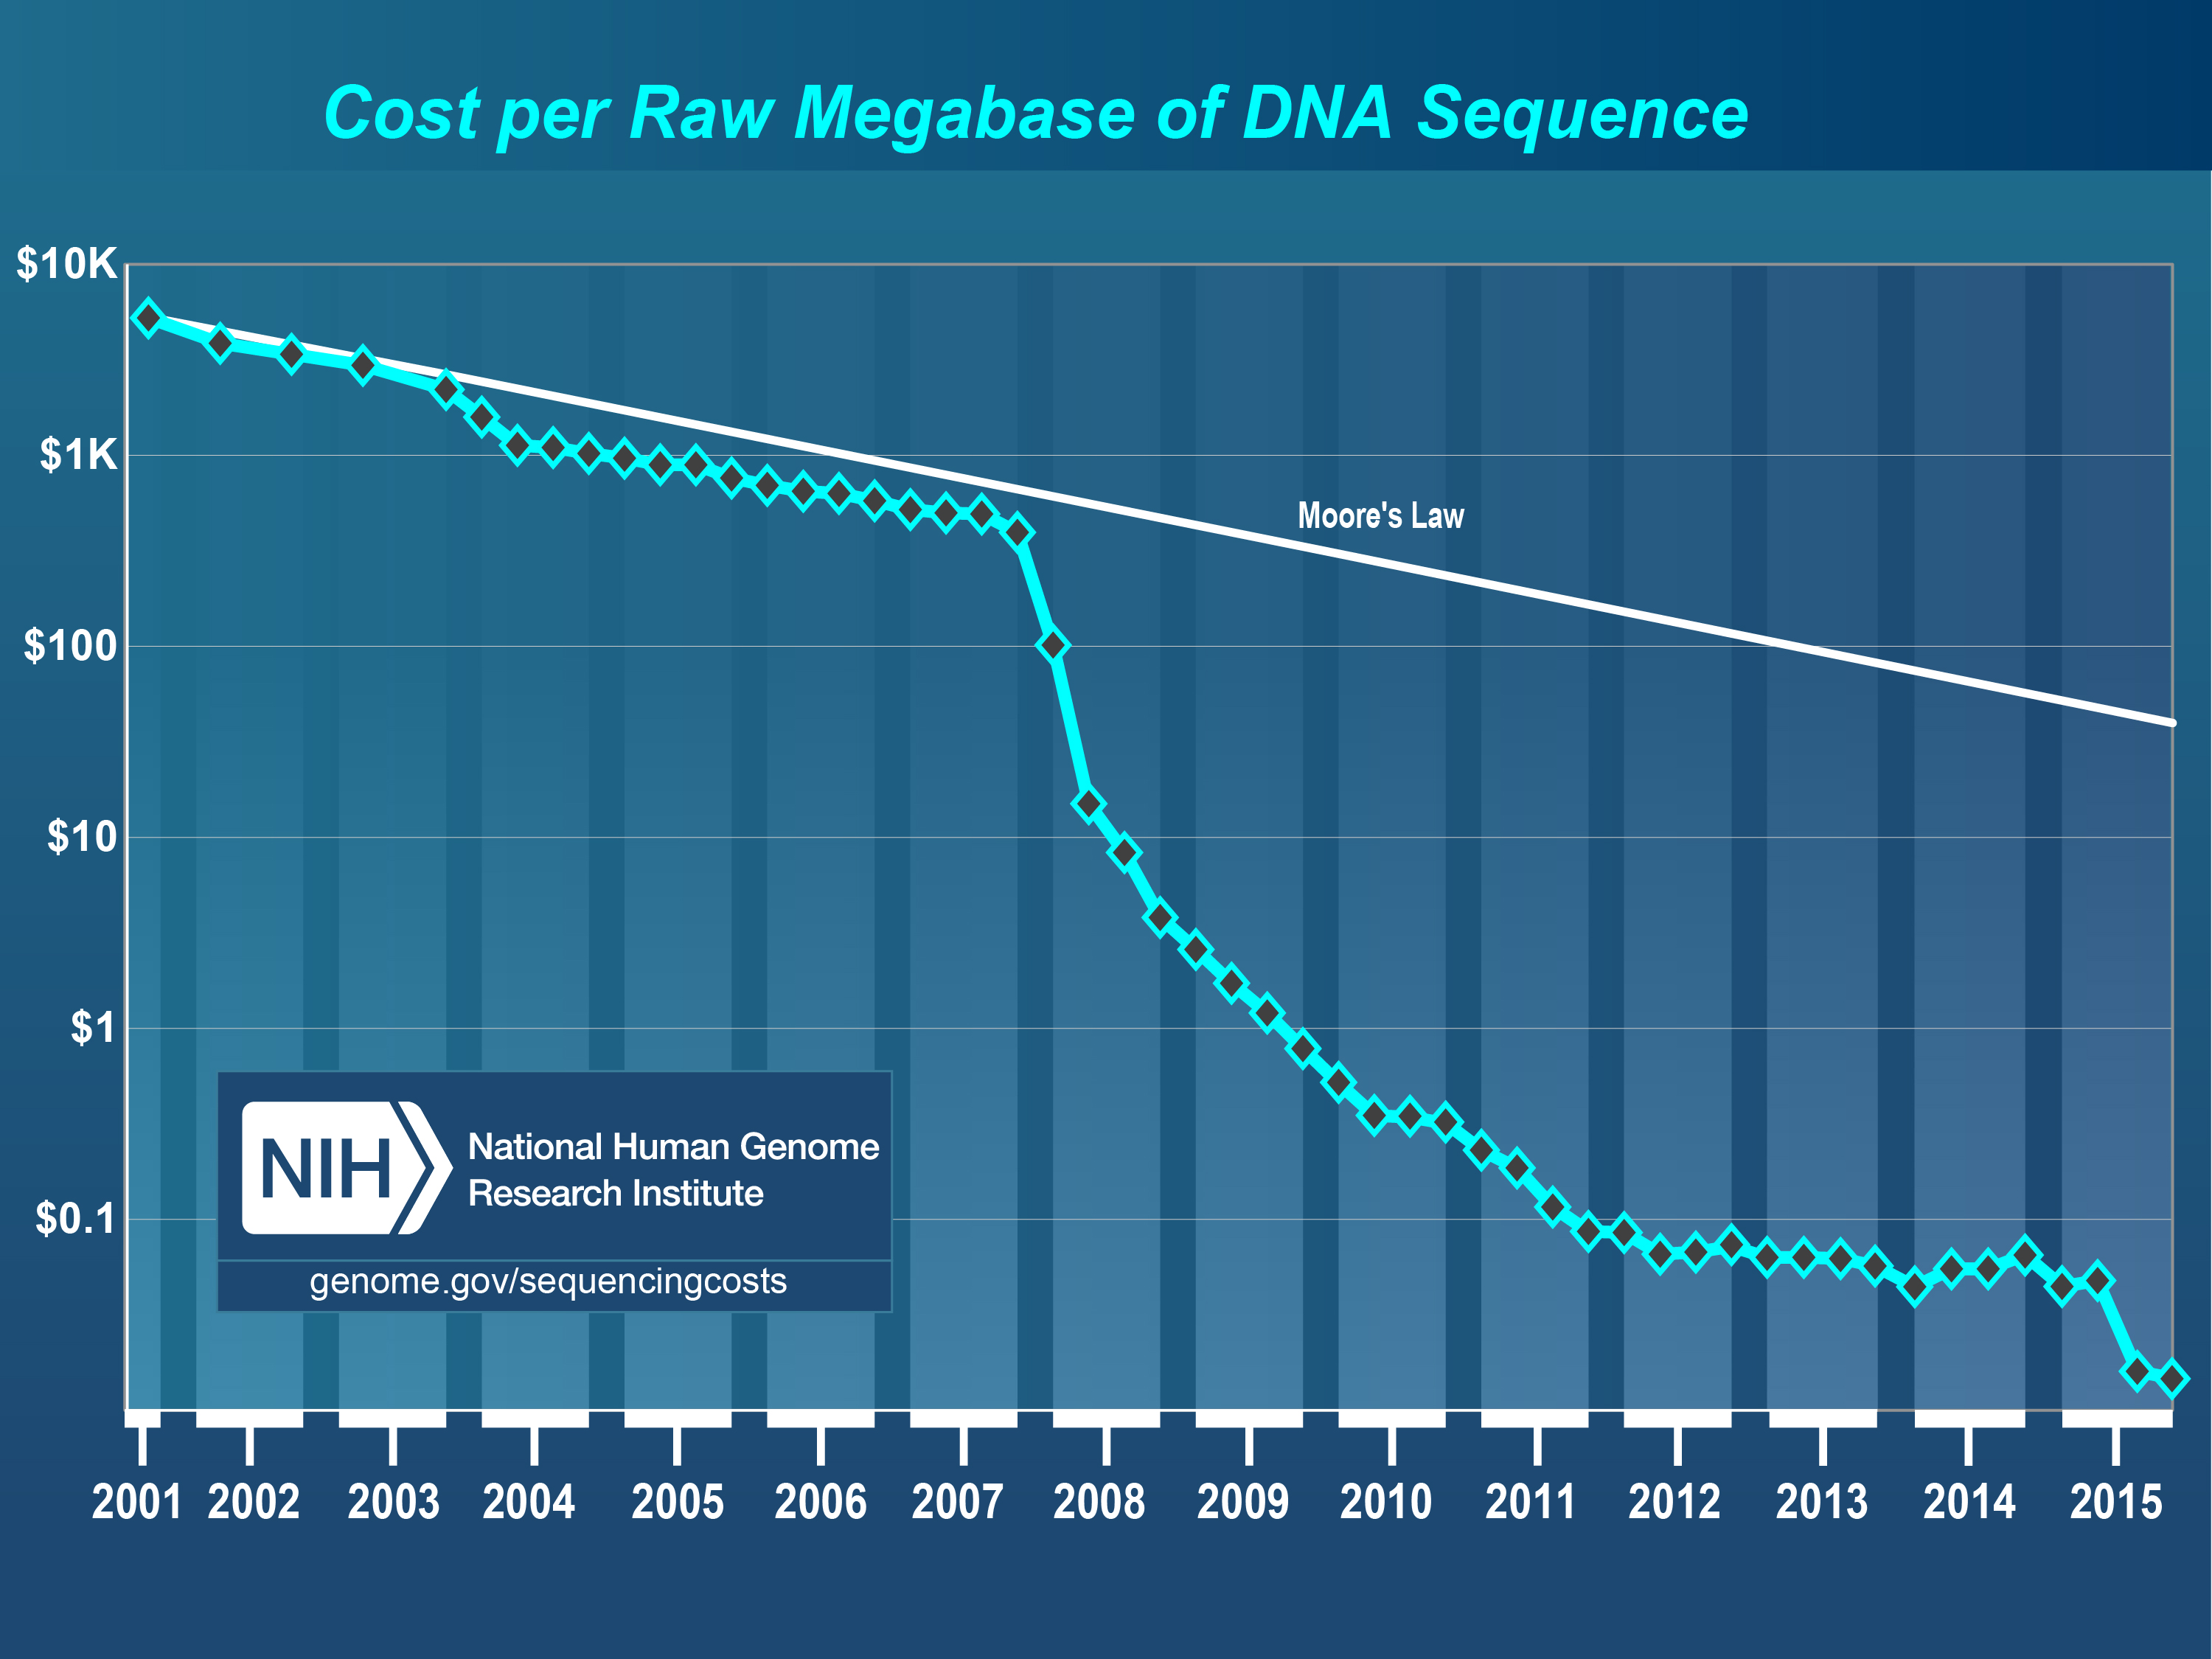
\includegraphics[scale=0.5]{costperMb2015_4.jpg}
% \end{center}
% \caption[Cost per raw megabase of DNA sequence from 2001 to 2015]{Cost per raw megabase of DNA sequence from 2001 to 2015. Straight line - Moore's Law, blue curve - cost in US dollars, Y-axis scale is logarithmic. Graph reproduced from ]{}
% \end{figure}



\end{document}
